\documentclass[border=5pt]{standalone}
\usepackage{fontspec,graphicx,tikz}
\setmainfont{FiraSans-Regular.otf}[BoldFont=FiraSans-Bold.otf]
\definecolor{ink}{HTML}{0E3B38}
\definecolor{pgreen}{HTML}{446F4E}
\definecolor{firered}{HTML}{D12632}
\definecolor{gray}{HTML}{CFE3E1}
\definecolor{grid}{HTML}{E1EEED}
\begin{document}\color{ink}
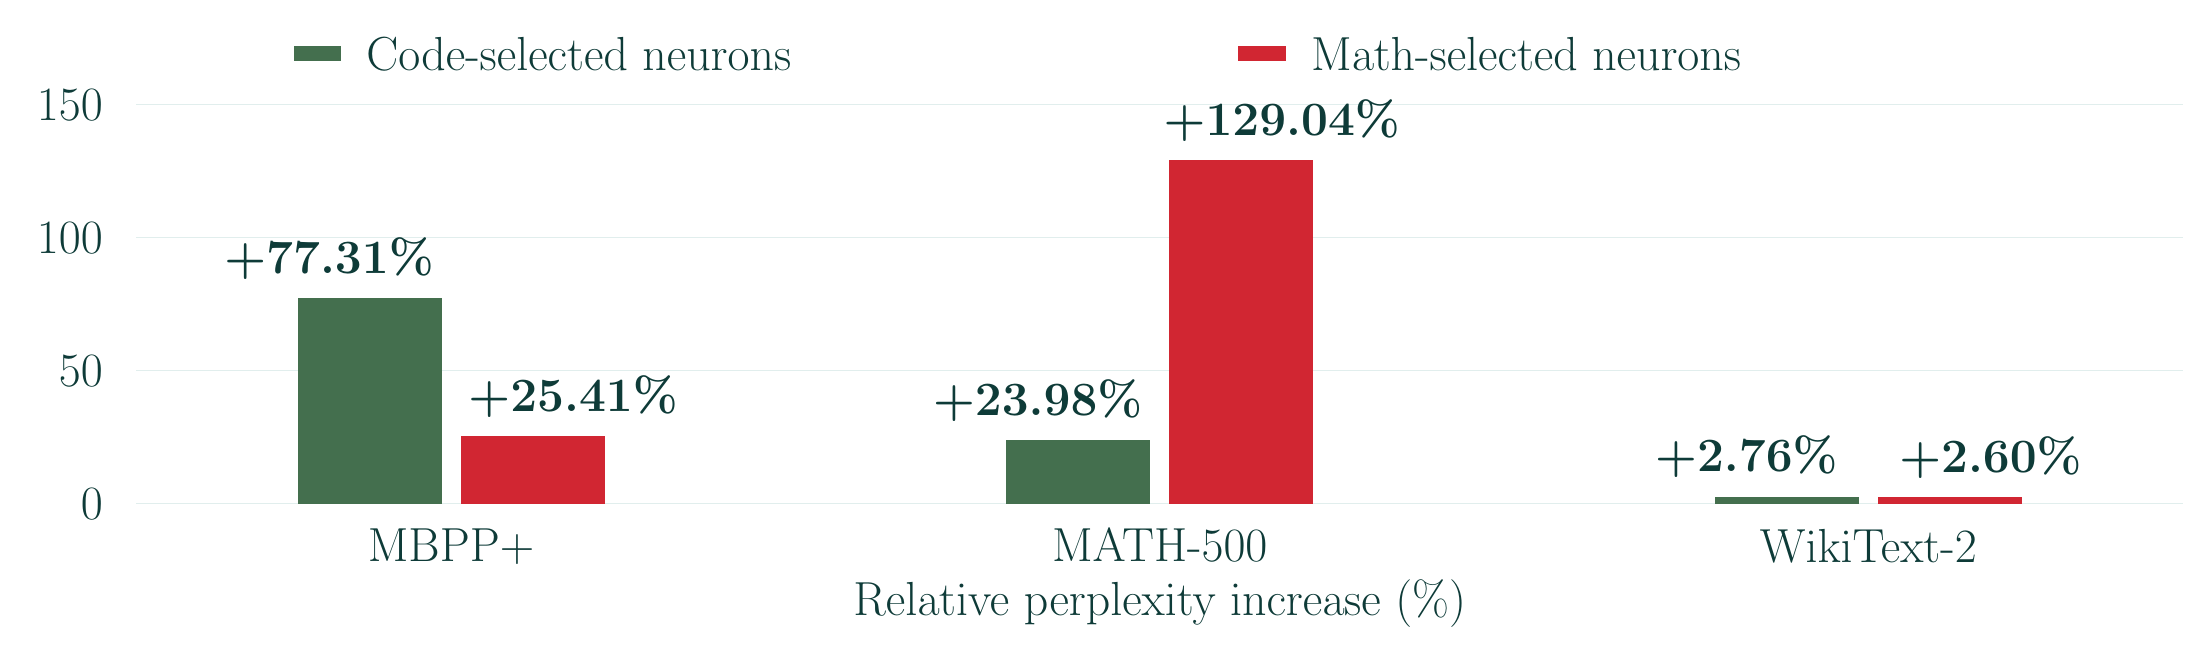
\begin{tikzpicture}[x=1cm,y=.65cm,every node/.style={font=\fontsize{18}{22}\selectfont}]
\draw[grid] (1,0.000) -- (27,0.000);
\node[anchor=east,text=ink,font=\fontsize{16}{20}\selectfont] at (0.700,0.000) {0};
\draw[grid] (1,2.600) -- (27,2.600);
\node[anchor=east,text=ink,font=\fontsize{16}{20}\selectfont] at (0.700,2.600) {50};
\draw[grid] (1,5.200) -- (27,5.200);
\node[anchor=east,text=ink,font=\fontsize{16}{20}\selectfont] at (0.700,5.200) {100};
\draw[grid] (1,7.800) -- (27,7.800);
\node[anchor=east,text=ink,font=\fontsize{16}{20}\selectfont] at (0.700,7.800) {150};
\path[fill=pgreen] (3.050,0.000) rectangle (4.880,4.020);
\path[fill=firered] (5.120,0.000) rectangle (6.950,1.321);
\node[anchor=south,text=ink,font=\fontsize{17}{21}\selectfont\bfseries] at (3.450,4.200) {+77.31\%};
\node[anchor=south,text=ink,font=\fontsize{17}{21}\selectfont\bfseries] at (6.550,1.501) {+25.41\%};
\node[anchor=north,text=ink,font=\fontsize{19}{23}\selectfont] at (5.000,-0.300) {MBPP+};
\path[fill=pgreen] (12.050,0.000) rectangle (13.880,1.247);
\path[fill=firered] (14.120,0.000) rectangle (15.950,6.710);
\node[anchor=south,text=ink,font=\fontsize{17}{21}\selectfont\bfseries] at (12.450,1.427) {+23.98\%};
\node[anchor=south,text=ink,font=\fontsize{17}{21}\selectfont\bfseries] at (15.550,6.890) {+129.04\%};
\node[anchor=north,text=ink,font=\fontsize{19}{23}\selectfont] at (14.000,-0.300) {MATH-500};
\path[fill=pgreen] (21.050,0.000) rectangle (22.880,0.144);
\path[fill=firered] (23.120,0.000) rectangle (24.950,0.135);
\node[anchor=south,text=ink,font=\fontsize{17}{21}\selectfont\bfseries] at (21.450,0.324) {+2.76\%};
\node[anchor=south,text=ink,font=\fontsize{17}{21}\selectfont\bfseries] at (24.550,0.315) {+2.60\%};
\node[anchor=north,text=ink,font=\fontsize{19}{23}\selectfont] at (23.000,-0.300) {WikiText-2};
\path[fill=pgreen] (3.000,8.660) rectangle (3.600,8.940);
\node[anchor=west,text=ink,font=\fontsize{17}{21}\selectfont] at (3.800,8.800) {Code-selected neurons};
\path[fill=firered] (15.000,8.660) rectangle (15.600,8.940);
\node[anchor=west,text=ink,font=\fontsize{17}{21}\selectfont] at (15.800,8.800) {Math-selected neurons};
\node[anchor=center,text=ink,font=\fontsize{19}{23}\selectfont] at (14.000,-1.950) {Relative perplexity increase (\%)};
\end{tikzpicture}\end{document}